% UG-MARL architecture diagram (ROADMAP 9.5). Build:
%   latexmk -pdf -outdir=build figures/architecture.tex   (from report/)
\documentclass[tikz,border=4pt]{standalone}
\usepackage[T1]{fontenc}
\usepackage{helvet}
\usepackage{amsmath,amssymb}
\renewcommand{\familydefault}{\sfdefault}
\usetikzlibrary{arrows.meta,positioning,fit,backgrounds,calc}

\definecolor{cdata}{HTML}{EEF0F2}
\definecolor{cinf}{HTML}{DCE9F7}
\definecolor{cinfline}{HTML}{2B6CB0}
\definecolor{ctrain}{HTML}{FCE8D5}
\definecolor{ctrainline}{HTML}{C05621}
\definecolor{cmp}{HTML}{E3F1E1}
\definecolor{cmpline}{HTML}{2F7D32}

\begin{document}
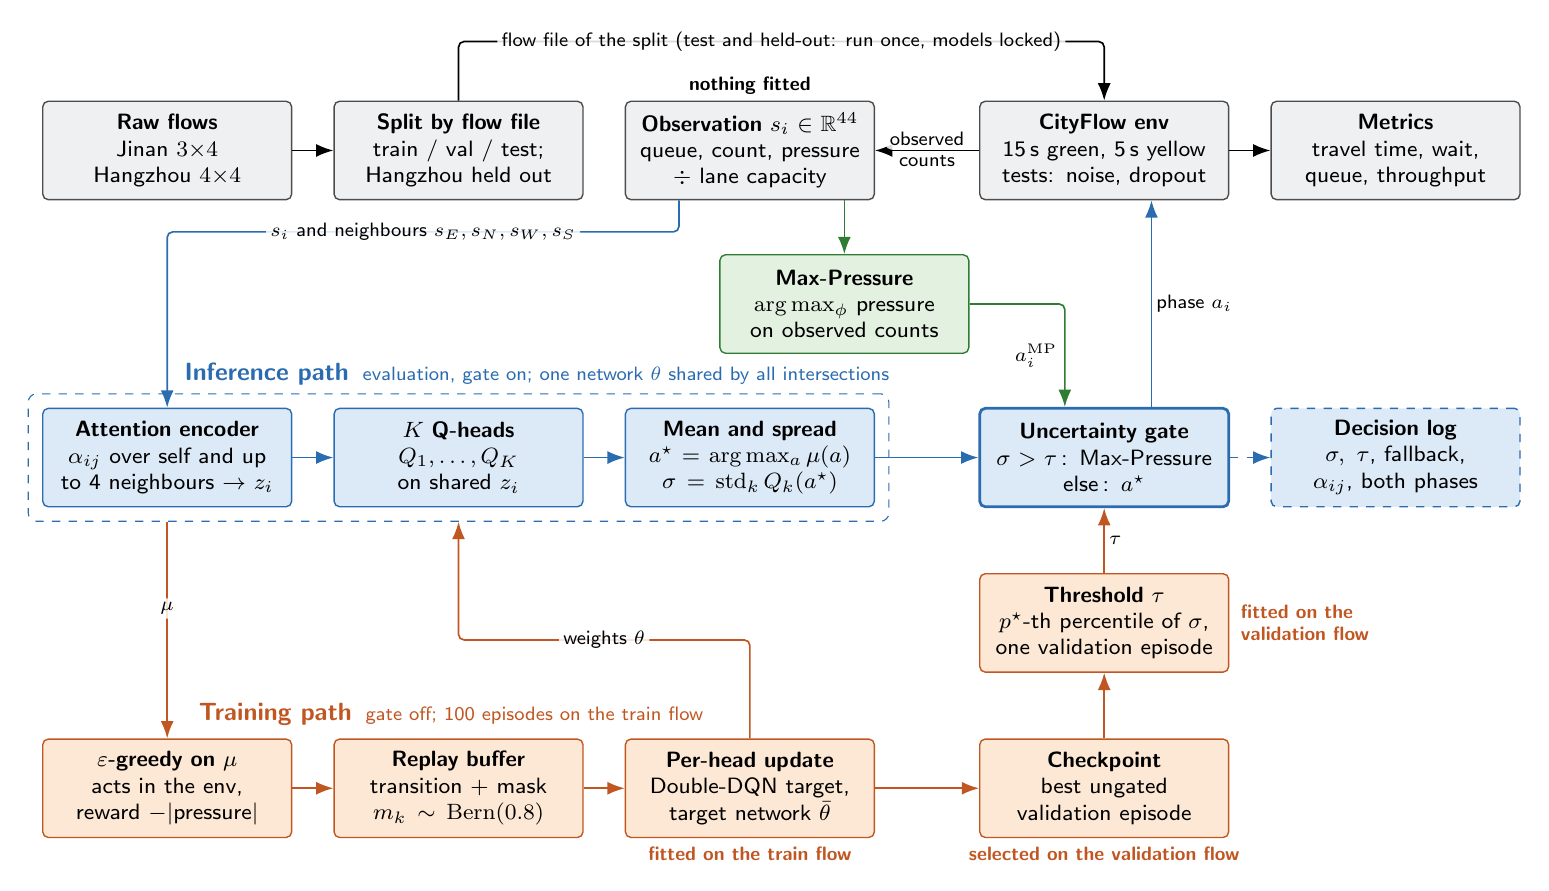
\begin{tikzpicture}[
    font=\footnotesize,
    box/.style={draw=black!70, rounded corners=2pt, align=center, text width=2.95cm,
                minimum height=1.25cm, inner sep=3pt, line width=0.5pt},
    data/.style={box, fill=cdata},
    inf/.style={box, fill=cinf, draw=cinfline},
    trn/.style={box, fill=ctrain, draw=ctrainline},
    mp/.style={box, fill=cmp, draw=cmpline},
    arr/.style={-{Latex[length=2.2mm]}, line width=0.6pt, rounded corners=2pt},
    iarr/.style={arr, draw=cinfline},
    tarr/.style={arr, draw=ctrainline},
    lab/.style={font=\scriptsize, inner sep=1.5pt, fill=white, fill opacity=0.85, text opacity=1},
    tag/.style={font=\scriptsize\bfseries, inner sep=1pt},
    lane/.style={font=\small\bfseries, align=left, text width=2.5cm},
]

% ---------------- data row ----------------
\node[data] (raw)   at (0,0)    {\textbf{Raw flows}\\Jinan $3{\times}4$\\Hangzhou $4{\times}4$};
\node[data] (split) at (3.7,0)  {\textbf{Split by flow file}\\train / val / test;\\Hangzhou held out};
\node[data] (obs)   at (7.4,0)  {\textbf{Observation} $s_i\in\mathbb{R}^{44}$\\queue, count, pressure\\$\div$ lane capacity};
\node[data] (env)   at (11.9,0) {\textbf{CityFlow env}\\15\,s green, 5\,s yellow\\tests: noise, dropout};
\node[data] (met)   at (15.6,0) {\textbf{Metrics}\\travel time, wait,\\queue, throughput};

\node[tag, above=1pt of obs.north] {nothing fitted};

\draw[arr] (raw) -- (split);
\draw[arr] (split.north) -- ++(0,0.75) -| node[lab, pos=0.25] {flow file of the split (test and held-out: run once, models locked)} (env.north);
\draw[arr] (env) -- node[lab, above] {observed} node[lab, below] {counts} (obs);
\draw[arr] (env) -- (met);

% ---------------- inference row ----------------
\node[inf] (enc)   at (0,-3.9)    {\textbf{Attention encoder}\\$\alpha_{ij}$ over self and up\\to 4 neighbours $\rightarrow z_i$};
\node[inf] (heads) at (3.7,-3.9)  {\textbf{$K$ Q-heads}\\$Q_1,\dots,Q_K$\\on shared $z_i$};
\node[inf] (mu)    at (7.4,-3.9)  {\textbf{Mean and spread}\\$a^\star=\arg\max_a \mu(a)$\\$\sigma=\mathrm{std}_k\,Q_k(a^\star)$};
\node[inf, line width=1pt] (gate) at (11.9,-3.9) {\textbf{Uncertainty gate}\\$\sigma>\tau$\,: Max-Pressure\\else\,: $a^\star$};
\node[inf, dashed] (log) at (15.6,-3.9) {\textbf{Decision log}\\$\sigma,\ \tau$, fallback,\\$\alpha_{ij}$, both phases};

\node[mp] (maxp) at (8.6,-1.95) {\textbf{Max-Pressure}\\$\arg\max_\phi$ pressure\\on observed counts};

\begin{scope}[on background layer]
  \node[draw=cinfline, dashed, rounded corners=3pt, inner sep=5pt, fit=(enc)(heads)(mu)] (net) {};
\end{scope}
\node[anchor=south west, text=cinfline, inner sep=1pt] at ($(net.north west)+(1.95,0.06)$)
  {\small\bfseries Inference path\enspace{\scriptsize\mdseries evaluation, gate on; one network $\theta$ shared by all intersections}};

\draw[iarr] ($(obs.south)+(-0.9,0)$) -- ++(0,-0.4) -| node[lab, pos=0.25] {$s_i$ and neighbours $s_E, s_N, s_W, s_S$} (enc.north);
\draw[arr, draw=cmpline] (maxp.north |- obs.south) -- (maxp.north);
\draw[iarr] (enc) -- (heads);
\draw[iarr] (heads) -- (mu);
\draw[iarr] (mu) -- (gate);
\draw[arr, draw=cmpline] (maxp.east) -| node[lab, pos=0.75, left=1pt] {$a^{\mathrm{MP}}_i$} ($(gate.north)+(-0.5,0)$);
\draw[iarr] ($(gate.north)+(0.6,0)$) -- node[lab, right, pos=0.5] {phase $a_i$} ($(env.south)+(0.6,0)$);
\draw[iarr, dashed] (gate) -- (log);

% ---------------- training row ----------------
\node[trn] (eps)  at (0,-8.1)    {\textbf{$\varepsilon$-greedy on $\mu$}\\acts in the env,\\reward $-|\text{pressure}|$};
\node[trn] (rep)  at (3.7,-8.1)  {\textbf{Replay buffer}\\transition + mask\\$m_k\sim\mathrm{Bern}(0.8)$};
\node[trn] (upd)  at (7.4,-8.1)  {\textbf{Per-head update}\\Double-DQN target,\\target network $\bar\theta$};
\node[trn] (ckpt) at (11.9,-8.1) {\textbf{Checkpoint}\\best ungated\\validation episode};
\node[trn] (tau)  at (11.9,-6.0) {\textbf{Threshold} $\tau$\\$p^\star$-th percentile of $\sigma$,\\one validation episode};

\draw[tarr] (eps.north |- net.south) -- node[lab, pos=0.4] {$\mu$} (eps.north);
\draw[tarr] (eps) -- (rep);
\draw[tarr] (rep) -- (upd);
\draw[tarr] (upd) -- (ckpt);
\draw[tarr] (upd.north) -- ++(0,1.25) -| node[lab, pos=0.25] {weights $\theta$} (heads.south |- net.south);
\draw[tarr] (ckpt) -- (tau);
\draw[tarr] (tau) -- node[lab, right] {$\tau$} (gate);

\node[anchor=south west, text=ctrainline, inner sep=1pt] at ($(eps.north west)+(1.95,0.12)$)
  {\small\bfseries Training path\enspace{\scriptsize\mdseries gate off; 100 episodes on the train flow}};

\node[tag, text=ctrainline, below=2pt of upd.south]  {fitted on the train flow};
\node[tag, text=ctrainline, below=2pt of ckpt.south] {selected on the validation flow};
\node[tag, text=ctrainline, right=3pt of tau.east, align=left] {fitted on the\\validation flow};

\end{tikzpicture}
\end{document}
